\documentclass[12pt]{beamer}
\usepackage[utf8]{inputenc}
\usetheme{Berkeley}
\usecolortheme{beaver}

\title{Decision Trees}
\author{Pattanin (Mill) Luangamornlert}
\institute{Durham University}
\date{\today}

\begin{document}

\frame{\titlepage}

\begin{frame}{Introduction}
   Decision Trees are a form of non-parametric statistics as well as machine learning. They show decision paths from a parent node to a child node to predict the likely outcome of an event given certain inputs.
   \begin{figure}
       \centering
       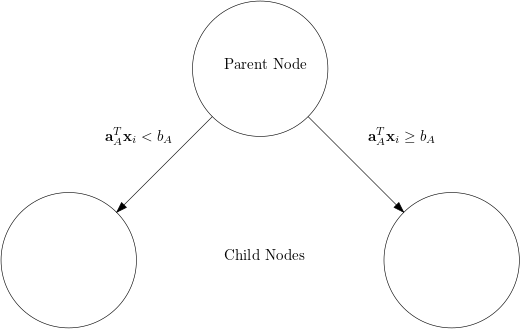
\includegraphics[width = 5cm]{ipefile/basicdt.png}
       \caption{A generic decision tree diagram}
       \label{fig:basicdt}
   \end{figure}
\end{frame}


\begin{frame}{History of Decision Trees}
    \begin{itemize}
        \item<1-> AID Algorithm \cite{AID}
        
        \item<2-> CHAID Algorithm \cite{CHAID}
        
        \item<3-> CART Algorithm \cite{BreimanDT}
        
        \item<4> ID3/C4.5 etc. \cite{Quinlan}
    \end{itemize}
\end{frame}

\begin{frame}{CART}
    CART was put together by Leo Breiman, Jerome Friedman, Richard Olshen, and Charles Stone in 1984 in their book, Classification and Regression Trees.\\
    It is the most popular method of Decision Trees today and is the basis of tree based machine learning methods.
\end{frame}

\begin{frame}{Splitting Metrics}
    
\end{frame}

\begin{frame}{Algorithm to Growing Trees}
    
\end{frame}

\begin{frame}{Pruning}
    
\end{frame}

\begin{frame}[allowframebreaks]
        \frametitle{References}
        \bibliographystyle{amsalpha}
        \bibliography{reference}
\end{frame}


\end{document}